\section{Implementierung}\label{kap_implementierung}

Im Rahmen einer Projektarbeit im Wintersemester 2014/15 wurde der in \cite{cima_paper} beschriebenen Algorithmus in einem Java-Applet implementiert. Ziel war es, den Algorithmus visuell darzustellen und ihn anhand des Applets in einem kurzen Vortrag vorzustellen.
\\
\\
Als Bestandteil dieser Bachelorarbeit haben wir das Applet mit der in Kapitel \ref{modifizierterAlgoChapter} beschriebenen Modifikation erweitert und die beiden Algorithmen in Kapitel \ref{kap_pot} entwickelt und ebenfalls in das Applet integriert.


\subsection{Benutzung des Applets}

Im Folgenden werden wir kurz beschreiben, wie das Applet benutzt werden kann:

\subsubsection*{Den Baum erstellen und ändern}

Man kann einen Baum (bzw. einen Baumknoten) erstellen, indem man mit einem Linksklick in das leere Applet klickt. Sofort erscheint ein Wurzelknoten.\\
Mit einem Linksklick auf einen Knoten fügt man ihm einen Kindknoten hinzu. Mit einem Rechtsklick auf einen Knoten wird dieser zusammen mit dem gesamten Teilbaum gelöscht.\\
Die Kantengewichte lassen sich ebenfalls mit einem Klick verändern. Ein Linksklick erhöht das entsprechende Kantengewicht um 1, ein Rechtsklick reduziert das Kantengewicht um 1. Allerdings können die Kantengewichte nicht kleiner als 1 werden.


\subsubsection*{Verwendung des Applets}

Nachdem man einen Baum erstellt hat, gibt es mehrere Funktionen, die man auswählen kann:\\

\begin{itemize}
	\item Man kann die Nachrichtenberechnung sowohl von dem ursprünglichen Algorithmus (Kapitel \ref{kap_algorithmus}), als auch von der Modifikation (Kapitel \ref{modifizierterAlgoChapter}) animieren lassen oder sofort das Ergebnis anzeigen. Bei der Animation wird immer angezeigt, wie jede einzelne Nachricht zustande kommt. Dies wird in Kurzform als Text und durch Färbung der einzelnen Elemente des Baumes verdeutlicht. Nachdem alle Nachrichten verschickt wurden, berechnet jeder Knoten, wie viele Agenten benötigt werden, um den gesamten Baum von diesen Knoten aus zu dekontaminieren. Dieser Wert wird am Ende in jedem Knoten angezeigt. Nach Abschluss des Algorithmus wird einer der Knoten mit minimaler Agentenzahl ausgewählt und als Homebase markiert.
	
	\item Alternativ zur Nachrichtenberechnung kann man sich die beiden Algorithmen aus Kapitel \ref{kap_pot} visuell darstellen lassen. Dazu werden ebenfalls die Nachrichten einzeln animiert (oder das Ergebnis sofort angezeigt), allerdings zeigen die Informationen (Text und Einfärbung), wie in jedem einzelnen Schritt die erweiterte Nachricht berechnet wird, die in dem jeweiligen Algorithmus benutzt wird. Man muss beachten, dass die Potentialberechnung nur mit der modifizierten Variante des Algorithmus ausführbar ist. Am Ende dieses Algorithmus wird angezeigt, wie viele Agenten jeder Knoten zu Dekontamination benötigt, welcher Knoten die Homebase ist, und, falls möglich, welche Kante reduziert werden sollte, um die Agentenzahl möglichst weit zu reduzieren.
	
	\item Außerdem lässt sich im Applet animieren, wie nach erfolgreicher Nachrichtenberechnung die Dekontamination des Baumes funktioniert. Die Strategie der Agenten ist dabei monoton. Dies bedeutet, dass jeder Knoten, der schon einmal dekontaminiert wurde, nicht mehr kontaminiert werden kann, da an den entsprechenden Stellen im Baum Wachen aufgestellt werden. Sind alle Knoten dekontaminiert, ist der Algorithmus abgeschlossen.
\end{itemize}

Alle Animationen können entweder als Ganzes abgespielt oder in einer Step-by-step-Animation in Teilen durchgeführt werden. \\
Alle Optionen, die im Applet verfügbar sind, werden eingeblendet. Alle in dem Moment nicht verfügbaren Optionen werden ausgeblendet, um eine bessere Übersicht zu gewährleisten.

\clearpage

\subsection{Beispiel aus dem Applet}





\begin{figure}[h]
	\subfigure[Verschiedene Einstellungs- und Nutzungsmöglichkeiten, welche das Applet bietet, sobald ein Baum erstellt wurde.
	\label{applet_a}]{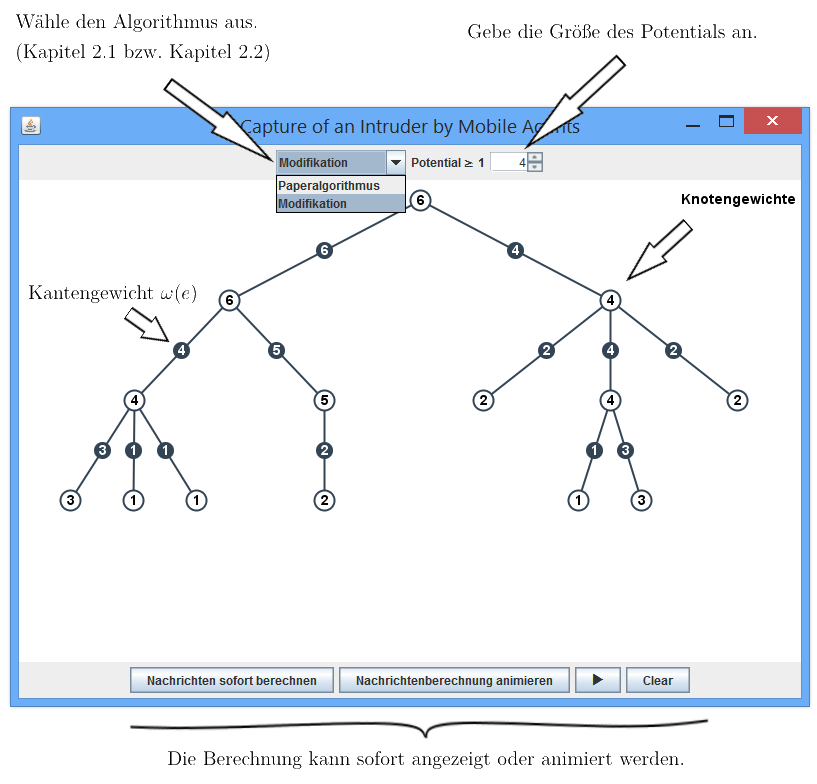
\includegraphics[width=0.85\textwidth]{bilder/abb_erklaerung1.png}}
	%	\hfill  
	%lösche die neue line und füge das \hfill wieder ein um die bilder nebeneiander zu haben
	
	\subfigure[Informationen über die aktuell berechnete Nachricht, bei allen Algorithmusvarianten (mit Potential oder ohne). \label{applet_b}]{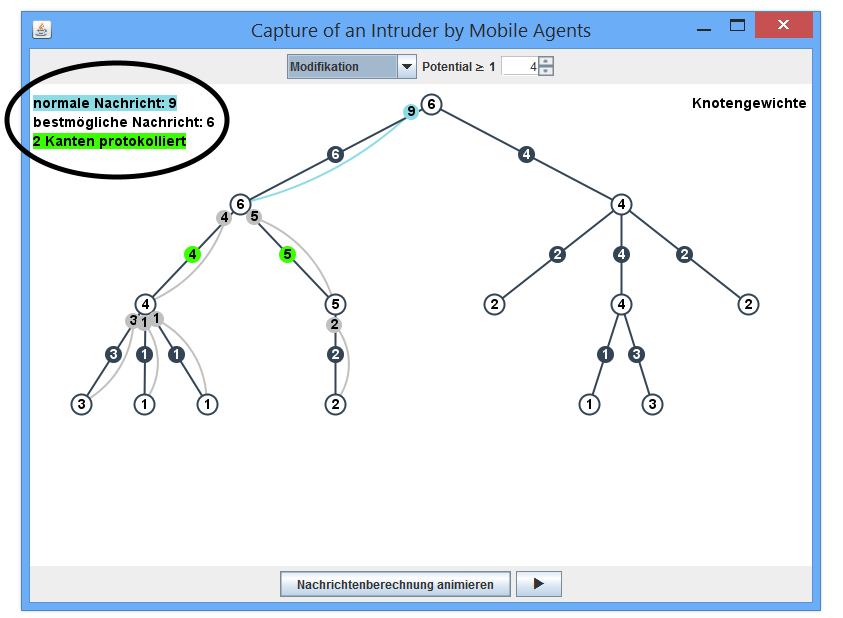
\includegraphics[width=0.85\textwidth]{bilder/abb_erklaerung2.png}} 
	%	\hfill
	
\end{figure}
\begin{figure}[h]
	
	\ContinuedFloat
	
	\subfigure[Nach der Berechnung wird das Ergebnis, auf welche Kanten das Potential eingesetzt werden kann, angezeigt. \label{applet_c}]{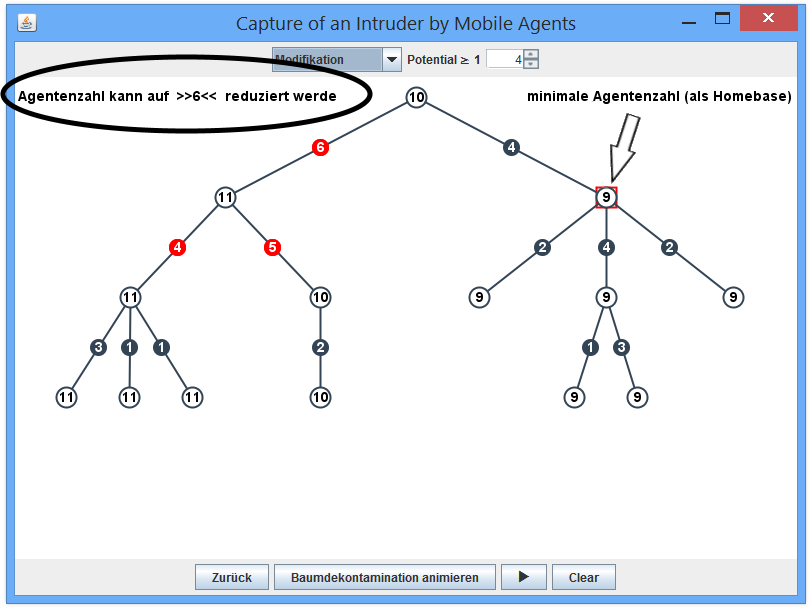
\includegraphics[width=0.85\textwidth]{bilder/abb_erklaerung3.png}}  
	
	\subfigure[Die Agenten dekontaminieren den Baum suzzessive. Dafür müssen an bestimmten Stellen Wachen aufgestellt werden. \label{applet_d}]{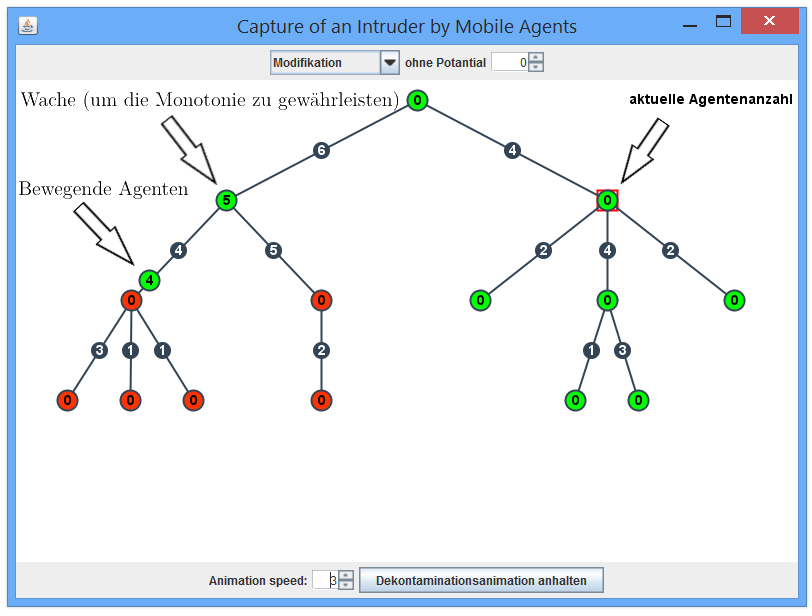
\includegraphics[width=0.85\textwidth]{bilder/abb_erklaerung4.png}}  
	
	\caption{Die Anwendung des Applets wird anhand eines Beispiels verdeutlicht.} 
	
\end{figure}	
